\documentclass[12pt]{article}
\usepackage{latexsym,amssymb,amsmath} 
\usepackage{cite}
\usepackage{path}
\usepackage{url}
\usepackage{verbatim}
\usepackage[pdftex]{graphicx}
\usepackage{fancyhdr}

\setlength{\oddsidemargin}{0.0in}
\setlength{\textwidth}{6.5in}
\setlength{\topmargin}{-1cm}
\setlength{\headheight}{12pt}
\setlength{\headsep}{25pt}
\setlength{\textheight}{625pt}
\setlength{\footskip}{24pt}

\renewcommand{\headrulewidth}{0pt}
\renewcommand{\textfraction}{0.10}
\renewcommand{\topfraction}{0.85}
\renewcommand{\bottomfraction}{0.85}
\renewcommand{\floatpagefraction}{0.90}

\numberwithin{equation}{section}
\numberwithin{table}{section}
\numberwithin{figure}{section}

\begin{document}
\DeclareGraphicsExtensions{.jpg}

%-------------------------Starts-------------------------------
\thispagestyle{fancy}
\rhead{$\mu$DBS Documentation}

\begin{center}
\textbf{\Large Process Fabrication for $\mu$DBS} \\[20pt]
  Daria Nesterovich\footnote{daria.nesterovich@utah.edu}\\[2pt] \emph{Salt Lake City, 84112, USA}  \\[6pt]
  (Dated: \today)
\end{center}

\vspace{6pt}


\begin{abstract}
The following content outlines the fabrication steps done in the Utah NanoFab Lab to build the $\mu$DBS. The purpose of this lab is to establish working recipes for the process and keep track of past failures.
\end{abstract}

\section{Design Process Overview}

\subsection{Design Architecture}

The fabrication of the $\mu$DBS begins with design in Cadence through the X-FAB XC06 design package. The design is sent to X-FAB Foundry (Erfurt, GE) for fabrication. The chips that are returned must undergo metal plating for the contacts and the bond pads, a parylene coating, dicing, wire bonding, and assembly. The design architecture can be found in Figure~\ref{DesignArchitecture}

\begin{figure} \centering
  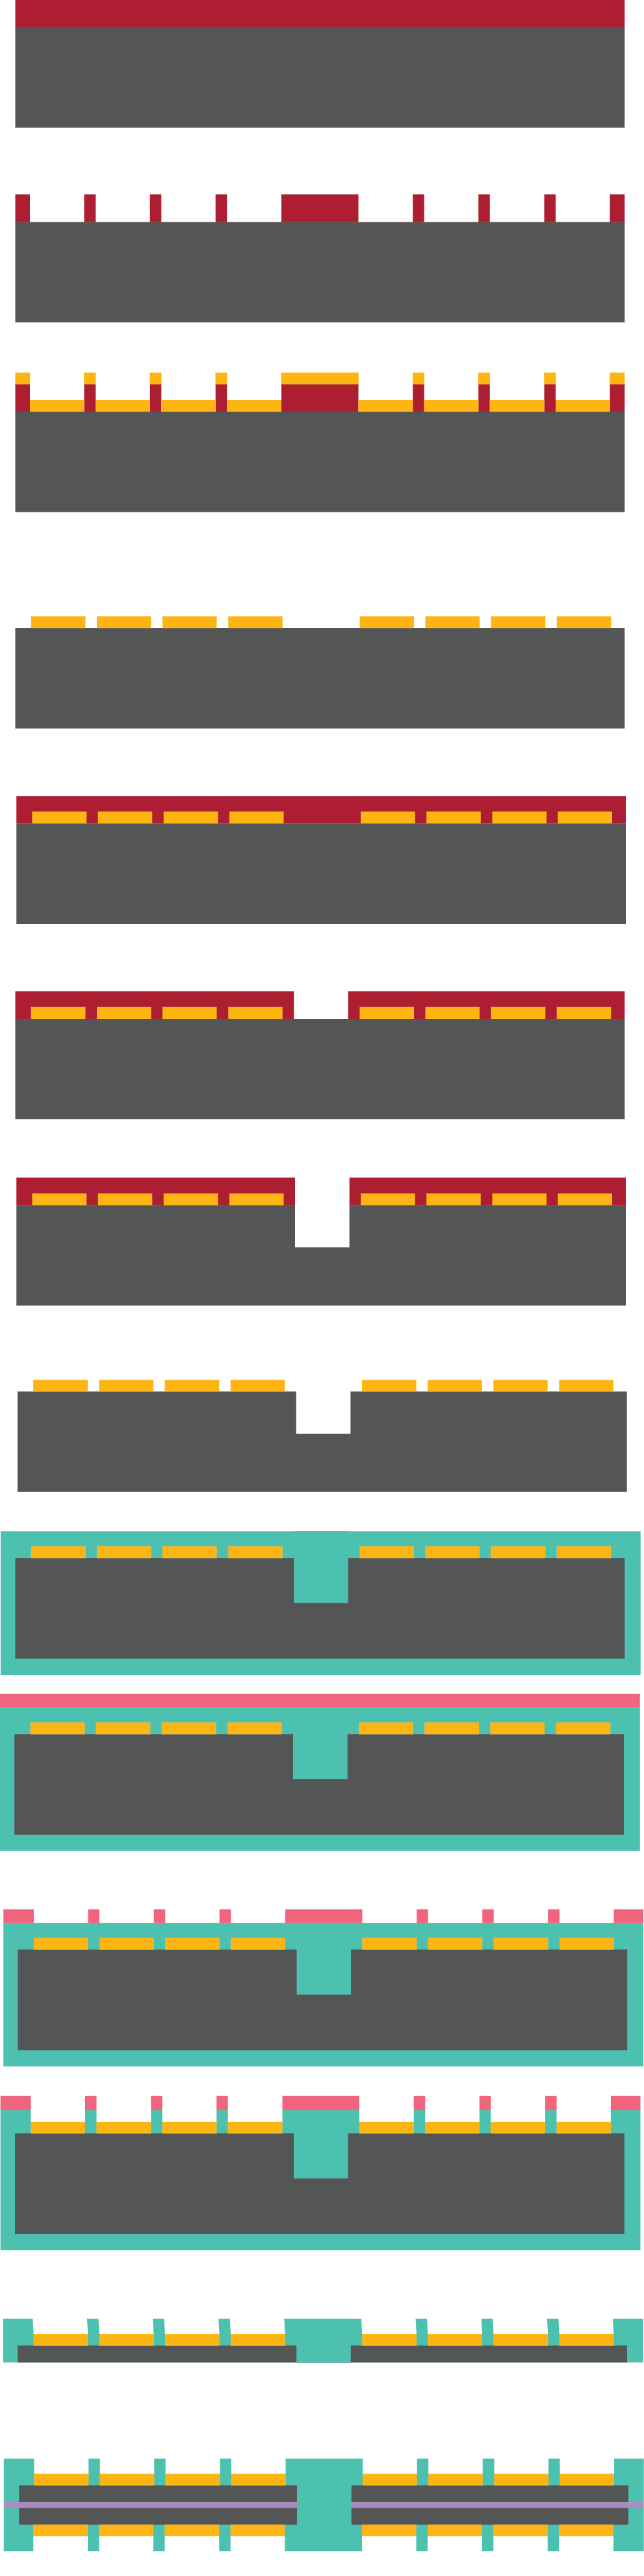
\includegraphics[width=0.25\textwidth]{DesignArchitecture.png}
  \caption{Design Architecture}
  \label{DesignArchitecture}
\end{figure}


\subsection{Another subsection}

For citing more than one paper, Please do like this
\cite{article1,article2,article3}. If you want to cite only a few chapters of a book, please do like this
\cite[Chapters~1--3]{book1}.

\section{Creation of Gold Contacts} 
\label{label1}

To refer a section, please use this: Section~\ref{label1}.

The equation can be done by:
\begin{align} 
	a = b+c.
	\label{eqn1}
\end{align}

Refer to the photo and equation can be done easily: Figure~\ref{Ao} and Equation~\ref{eqn1}.

You can also make a table like in Table~\ref{table1}:

\begin{table} \centering
  \begin{tabular}{r|c}
    \hline
    Process & e \\
    \hline
       RPM & 2000 \\
       Resist & 1813 \\
    \hline
  \end{tabular}
  \caption{This is a table.}
  \label{table1}
\end{table}

A figure with two subfigures on its left and right sides can be done in, for example, 
Figure~\ref{Aoprime}.

You can display any texts by:
\begin{verbatim}
\begin{figure} \centering
\end{figure}
\end{verbatim}

\section*{Acknowledgments}

This is where you want to thank some of your colleagues and friends. This is where you want to thank some of your colleagues and friends. This is where you want to thank some of your colleagues and friends. This is where you want to thank some of your colleagues and friends. This is where you want to thank some of your colleagues and friends. 
 
\appendix

\section{Appendix 1} 
\label{appendix_1}

This can be some appendix. This can be some appendix. This can be some appendix. This can be some appendix. This can be some appendix. This can be some appendix. This can be some appendix. This can be some appendix. This can be some appendix. This can be some appendix. This can be some appendix. 

%-------------------------Ends-------------------------------
\bibliographystyle{siam}
\bibliography{FermiTMtemp}

\end{document}

